% ============================================================
%  TERM PROJECT – PROPOSAL (template)
%  Databases · THGA Bochum
%
%  How to use:
%    1. Copy this folder into your own repository.
%    2. Replace every  <<< ... >>>  placeholder with your content.
%    3. Build with  `make`  (see the Makefile / README).
%    4. Send the resulting PDF to the lecturer and wait for approval.
% ============================================================
\documentclass[11pt,a4paper]{article}
\makeatletter
\def\input@path{{../style/}}
\makeatother
\usepackage{thga-db}

% ----- Fill in your metadata -------------------------------
\renewcommand{\thgaKurs}{Databases}
\renewcommand{\thgaDatum}{Summer Term 2026}
\newcommand{\authorName}{Niklas Stratenwerth}
\newcommand{\projectTitle}{Wartungsmanagement DB}

\begin{document}
\thispagestyle{empty}
\thgaTitel{Term Project – Proposal}{\projectTitle}

\begin{infobox}
\textbf{Author:} \authorName \\
\textbf{Module:} Introduction to Database Management Systems · THGA Bochum \\
\textbf{Submitted to:} Stephan Bökelmann · \href{mailto:sboekelmann@ep1.rub.de}{sboekelmann@ep1.rub.de} \\
\textbf{Target size:} 2--4 pages
\end{infobox}

% ============================================================
\section{Application domain and motivation}
% ============================================================

Wartungsmanagement 
Geräte, Wartungsplan, Wartung, Techniker, Standorte

Planen wann ein Gerät durch wen gewartet werden soll plant im vorraus, wann Wartungen
anstehen und weißt einen Techniker zu.
Festhalten wann es durch wen gewartet wurde, hierdurch kann man nachträglich
nachhalten, ob Wartungsintervalle eingehalten wurden und wer die letzte Wartung 
durchgeführt hat.

Geräte: haben ein Wartungsintervall und einen Standort
Wartungsplan: wann welches Gerät durch wen gewartet werden soll
Wartung: Durchgeführte Wartungen
Techniker: sind zuständig für Standorte und Gerätetypen
Standorte: betreut durch Techniker, haben verschiedene Geräte
% ============================================================
\section{Data model -- ER sketch}
% ============================================================



\begin{center}
  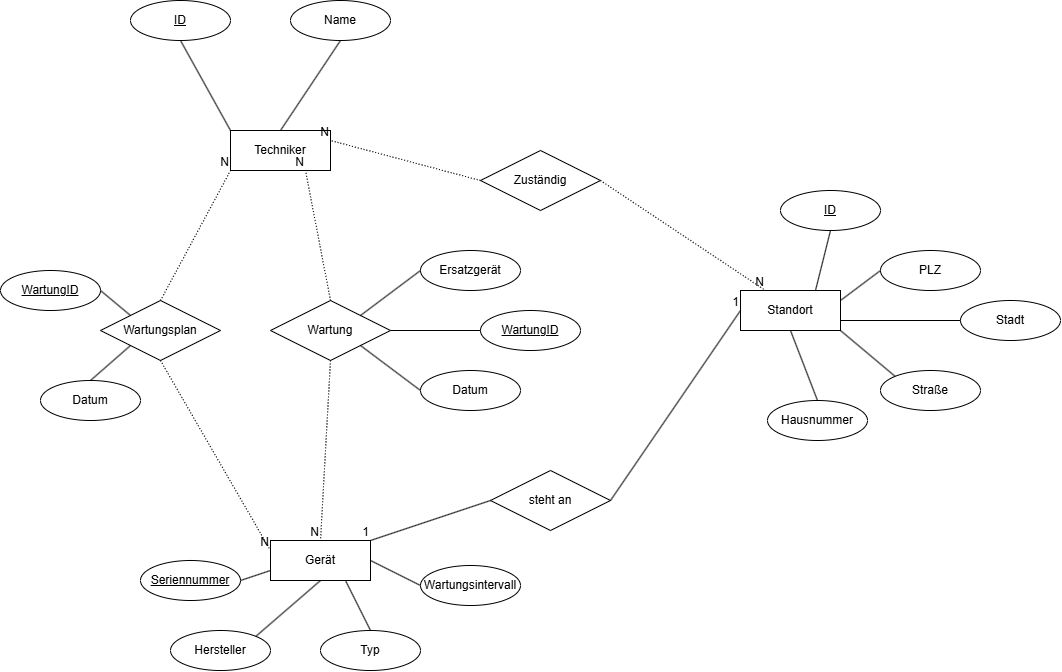
\includegraphics[width=0.9\linewidth]{ER-Sketch.drawio.png}
 \end{center}

% ============================================================
\section{From model to schema}
% ============================================================



\begin{center}
  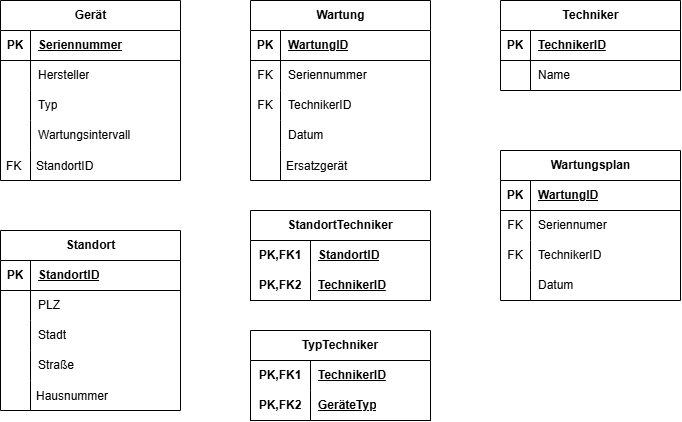
\includegraphics[width=0.9\linewidth]{Schema-Sketch.drawio.png}
 \end{center}

\textbf{Normalisation.} Das Schema ist in der 3. NF, da jedes nicht Schlüsselattribut nur vom Primärschlüssel abhängt. 
Alle N:M Beziehungen sind in separaten Tabellen, wodurch Redundanz vermieden wird 

% ============================================================
\section{API design}
% ============================================================



\renewcommand{\arraystretch}{1.2}
\begin{tabularx}{\linewidth}{@{}p{2cm}p{4cm}X@{}}
\toprule
\textbf{Method} & \textbf{Path} & \textbf{Purpose} \\
\midrule
\texttt{GET}    & \texttt{/techniker/\{id\}/wartungsplan} 
& Liefert die geplanten Wartungen eines Technikers mit Gerät und Standort (JOIN) \\

\texttt{GET}    & \texttt{/geraete/\{seriennummer\}/wartungen} 
& Liefert die Wartungshistorie eines Geräts mit den ausführenden Technikern (JOIN) \\

\texttt{GET}    & \texttt{/geraete/\{seriennummer\}} 
& Liefert Gerätedaten einschließlich Standort und nächster Wartung \\

\texttt{GET}    & \texttt{/standorte/\{id\}/geraete} 
& Liefert alle Geräte eines Standorts \\

\texttt{GET}    & \texttt{/wartungsplan?von=\{datum\}\&bis=\{datum\}} 
& Liefert alle geplanten Wartungen innerhalb eines Zeitraums \\

\texttt{GET}    & \texttt{/wartungsplan/ueberfaellig} 
& Liefert alle noch nicht durchgeführten und überfälligen Wartungen \\

\texttt{POST}   & \texttt{/wartungen} 
& Dokumentiert eine durchgeführte Wartung (requires X-API-Key) \\

\texttt{POST}   & \texttt{/geraete} 
& Erstellt ein neues Gerät (requires X-API-Key) \\

\texttt{POST}   & \texttt{/wartungsplan} 
& Plant eine Wartung für ein Gerät und einen Techniker (requires X-API-Key) \\

\texttt{PUT}    & \texttt{/wartungsplan/\{id\}} 
& Ändert Termin oder Techniker einer geplanten Wartung (requires X-API-Key) \\

\texttt{PATCH}  & \texttt{/geraete/\{seriennummer\}} 
& Ändert beispielsweise Standort oder Wartungsintervall eines Geräts (requires X-API-Key) \\

\texttt{DELETE} & \texttt{/wartungsplan/\{id\}} 
& Entfernt eine geplante Wartung (requires X-API-Key) \\

\texttt{GET} & \texttt{/statistik/wartungen-pro-techniker} 
& Anzahl der Wartungen je Techniker in einem Zeitraum (GROUP BY / aggregation) \\

\texttt{GET} & \texttt{/statistik/wartungen-pro-standort} 
& Anzahl durchgeführter und geplanter Wartungen je Standort (JOIN / aggregation) \\
\bottomrule
\end{tabularx}

% ============================================================
\section{Frontend idea}
% ============================================================

tkinter Frontend, 
Eintragen von neuen Geräten, Eintragen von Wartungen, 
Anschauen von Wartungen, Anschauen vom Wartungsplan für einen Techniker
statistik Seite, wo man sich Wartungen nach Standort oder Techniker Anschauen kann
Anschauen von überfälligen Wartungen
% ============================================================
\section{Operation with Docker Compose}
% ============================================================

docker-compose.yaml wird zwei Services haben, die PostgreSQL Datenbank 
und eine Backend Anwendung, welche für die api zuständig ist.

im .env werden die credentials und configuration values der Datenbank gespeichert.
Es wird nur ein .env.example committed, welches als Beispiel dient. 

Das Projekt wird auf den Server kopiert und über \texttt{docker compose up -d --build} gestartet.

% ============================================================
\section{Scope, milestones and risks}
% ============================================================

\textbf{Scope.} 7 Tables, 14 Api Points

\textbf{Milestones.}
\begin{enumerate}[topsep=2pt]
  \item  Database ready: 1 Week, 15 hours
  \item  API ready: 2 days, 7 Hours
  \item frontend operates the core endpoints, packaged as .deb: 10 days, 15 hours
  \item documentation + video:  1 day, 3 Hours
\end{enumerate}

\textbf{Risks.} 
Database or Frontend could take longer to implement

\vspace{1em}
\begin{infobox}
\textbf{Effort budget:} the whole term project (system, documentation and video)
should fit into roughly \textbf{40\,h of work} over at most \textbf{2 months}.
Keep your scope within that budget.
\end{infobox}

\end{document}
